%%%%%%%%%%%%%%%%%%%%%%%%%%%%%%%%%%%%%%%%%
%  My documentation report
%  Objetive: Explain what I did and how, so someone can continue with the investigation
%
% Important note:
% Chapter heading images should have a 2:1 width:height ratio,
% e.g. 920px width and 460px height.
%
%%%%%%%%%%%%%%%%%%%%%%%%%%%%%%%%%%%%%%%%%

%----------------------------------------------------------------------------------------
%	PACKAGES AND OTHER DOCUMENT CONFIGURATIONS
%----------------------------------------------------------------------------------------

\documentclass[11pt,fleqn]{book} % Default font size and left-justified equations

\usepackage[top=3cm,bottom=3cm,left=3.2cm,right=3.2cm,headsep=10pt,letterpaper]{geometry} % Page margins

\usepackage{xcolor,lipsum} % Required for specifying colors by name
\definecolor{ocre}{RGB}{73,73,73} 
\definecolor{lightgray}{RGB}{229,229,229} 
% Font Settings
\usepackage{avant} % Use the Avantgarde font for headings
%\usepackage{times} % Use the Times font for headings
\usepackage{mathptmx} % Use the Adobe Times Roman as the default text font together with math symbols from the Sym­bol, Chancery and Com­puter Modern fonts

\usepackage{microtype} % Slightly tweak font spacing for aesthetics
\usepackage[utf8]{inputenc} % Required for including letters with accents
\usepackage[T1]{fontenc} % Use 8-bit encoding that has 256 glyphs


% MATHS PACKAGE
\usepackage{amsmath,tikz}
\usetikzlibrary{matrix}
\usetikzlibrary{calc}
\usetikzlibrary{shapes}
\usetikzlibrary{backgrounds,fit,shapes}
\usetikzlibrary{positioning}

\newcommand*{\horzbar}{\rule[0.05ex]{2.5ex}{0.5pt}}
\usepackage{calc}

% VERBATIM PACKAGE
\usepackage{verbatim}

% Bibliography
%\usepackage[style=alphabetic,sorting=nyt,sortcites=true,autopunct=true,babel=hyphen,hyperref=true,abbreviate=false,backref=true,backend=biber]{ieeetran}

%\addbibresource{bibliography.bib} % BibTeX bibliography file
%\defbibheading{bibempty}{}

%----------------------------------------------------------------------------------------
%	VARIOUS REQUIRED PACKAGES
%----------------------------------------------------------------------------------------

\usepackage[top=3cm,bottom=3cm,left=3.2cm,right=3.2cm,headsep=10pt,letterpaper]{geometry} % Page margins

\usepackage{titlesec} % Allows customization of titles

\usepackage{graphicx} % Required for including pictures
\graphicspath{{Pictures/}} % Specifies the directory where pictures are stored

\usepackage{lipsum} % Inserts dummy text

\usepackage{tikz} % Required for drawing custom shapes

\usepackage[english]{babel} % English language/hyphenation

\usepackage{enumitem} % Customize lists
\setlist{nolistsep} % Reduce spacing between bullet points and numbered lists

\usepackage{booktabs} % Required for nicer horizontal rules in tables

\usepackage{eso-pic} % Required for specifying an image background in the title page

\usepackage{xcolor,lipsum} % Required for specifying colors by name
\definecolor{gridcal_green}{RGB}{0,170,136}
\definecolor{gridcal_green2}{RGB}{0,170,170}
%----------------------------------------------------------------------------------------
%	MAIN TABLE OF CONTENTS
%----------------------------------------------------------------------------------------

\usepackage{titletoc} % Required for manipulating the table of contents

\contentsmargin{0cm} % Removes the default margin
% Chapter text styling
\titlecontents{chapter}[1.25cm] % Indentation
{\addvspace{15pt}\large\sffamily\bfseries} % Spacing and font options for chapters
{\color{ocre!60}\contentslabel[\Large\thecontentslabel]{1.25cm}\color{ocre}} % Chapter number
{}  
{\color{ocre!60}\normalsize\sffamily\bfseries\;\titlerule*[.5pc]{.}\;\thecontentspage} % Page number
% Section text styling
\titlecontents{section}[1.25cm] % Indentation
{\addvspace{5pt}\sffamily\bfseries} % Spacing and font options for sections
{\contentslabel[\thecontentslabel]{1.25cm}} % Section number
{}
{\sffamily\hfill\color{black}\thecontentspage} % Page number
[]
% Subsection text styling
\titlecontents{subsection}[1.25cm] % Indentation
{\addvspace{1pt}\sffamily\small} % Spacing and font options for subsections
{\contentslabel[\thecontentslabel]{1.25cm}} % Subsection number
{}
{\sffamily\;\titlerule*[.5pc]{.}\;\thecontentspage} % Page number
[] 

%----------------------------------------------------------------------------------------
%	MINI TABLE OF CONTENTS IN CHAPTER HEADS
%----------------------------------------------------------------------------------------

% Section text styling
\titlecontents{lsection}[0em] % Indendating
{\footnotesize\sffamily} % Font settings
{}
{}
{}

% Subsection text styling
\titlecontents{lsubsection}[.5em] % Indentation
{\normalfont\footnotesize\sffamily} % Font settings
{}
{}
{}
 
%----------------------------------------------------------------------------------------
%	PAGE HEADERS
%----------------------------------------------------------------------------------------

\usepackage{fancyhdr} % Required for header and footer configuration

\pagestyle{fancy}
\renewcommand{\chaptermark}[1]{\markboth{\sffamily\normalsize\bfseries\chaptername\ \thechapter.\ #1}{}} % Chapter text font settings
\renewcommand{\sectionmark}[1]{\markright{\sffamily\normalsize\thesection\hspace{5pt}#1}{}} % Section text font settings
\fancyhf{} \fancyhead[LE,RO]{\sffamily\normalsize\thepage} % Font setting for the page number in the header
\fancyhead[LO]{\rightmark} % Print the nearest section name on the left side of odd pages
\fancyhead[RE]{\leftmark} % Print the current chapter name on the right side of even pages
\renewcommand{\headrulewidth}{0.5pt} % Width of the rule under the header
\addtolength{\headheight}{2.5pt} % Increase the spacing around the header slightly
\renewcommand{\footrulewidth}{0pt} % Removes the rule in the footer
\fancypagestyle{plain}{\fancyhead{}\renewcommand{\headrulewidth}{0pt}} % Style for when a plain pagestyle is specified

% Removes the header from odd empty pages at the end of chapters
\makeatletter
\renewcommand{\cleardoublepage}{
\clearpage\ifodd\c@page\else
\hbox{}
\vspace*{\fill}
\thispagestyle{empty}
\newpage
\fi}

%----------------------------------------------------------------------------------------
%	THEOREM STYLES
%----------------------------------------------------------------------------------------

\usepackage{amsmath,amsfonts,amssymb,amsthm} % For math equations, theorems, symbols, etc

\newcommand{\intoo}[2]{\mathopen{]}#1\,;#2\mathclose{[}}
\newcommand{\ud}{\mathop{\mathrm{{}d}}\mathopen{}}
\newcommand{\intff}[2]{\mathopen{[}#1\,;#2\mathclose{]}}
\newtheorem{notation}{Notation}[chapter]

%%%%%%%%%%%%%%%%%%%%%%%%%%%%%%%%%%%%%%%%%%%%%%%%%%%%%%%%%%%%%%%%%%%%%%%%%%%
%%%%%%%%%%%%%%%%%%%% dedicated to boxed/framed environements %%%%%%%%%%%%%%
%%%%%%%%%%%%%%%%%%%%%%%%%%%%%%%%%%%%%%%%%%%%%%%%%%%%%%%%%%%%%%%%%%%%%%%%%%%
\newtheoremstyle{ocrenumbox}% % Theorem style name
{0pt}% Space above
{0pt}% Space below
{\normalfont}% % Body font
{}% Indent amount
{\small\bf\sffamily\color{ocre}}% % Theorem head font
{\;}% Punctuation after theorem head
{0.25em}% Space after theorem head
{\small\sffamily\color{ocre}\thmname{#1}\nobreakspace\thmnumber{\@ifnotempty{#1}{}\@upn{#2}}% Theorem text (e.g. Theorem 2.1)
\thmnote{\nobreakspace\the\thm@notefont\sffamily\bfseries\color{black}---\nobreakspace#3.}} % Optional theorem note
\renewcommand{\qedsymbol}{$\blacksquare$}% Optional qed square

\newtheoremstyle{blacknumex}% Theorem style name
{5pt}% Space above
{5pt}% Space below
{\normalfont}% Body font
{} % Indent amount
{\small\bf\sffamily}% Theorem head font
{\;}% Punctuation after theorem head
{0.25em}% Space after theorem head
{\small\sffamily{\tiny\ensuremath{\blacksquare}}\nobreakspace\thmname{#1}\nobreakspace\thmnumber{\@ifnotempty{#1}{}\@upn{#2}}% Theorem text (e.g. Theorem 2.1)
\thmnote{\nobreakspace\the\thm@notefont\sffamily\bfseries---\nobreakspace#3.}}% Optional theorem note

\newtheoremstyle{blacknumbox} % Theorem style name
{0pt}% Space above
{0pt}% Space below
{\normalfont}% Body font
{}% Indent amount
{\small\bf\sffamily}% Theorem head font
{\;}% Punctuation after theorem head
{0.25em}% Space after theorem head
{\small\sffamily\thmname{#1}\nobreakspace\thmnumber{\@ifnotempty{#1}{}\@upn{#2}}% Theorem text (e.g. Theorem 2.1)
\thmnote{\nobreakspace\the\thm@notefont\sffamily\bfseries---\nobreakspace#3.}}% Optional theorem note

%%%%%%%%%%%%%%%%%%%%%%%%%%%%%%%%%%%%%%%%%%%%%%%%%%%%%%%%%%%%%%%%%%%%%%%%%%%
%%%%%%%%%%%%% dedicated to non-boxed/non-framed environements %%%%%%%%%%%%%
%%%%%%%%%%%%%%%%%%%%%%%%%%%%%%%%%%%%%%%%%%%%%%%%%%%%%%%%%%%%%%%%%%%%%%%%%%%
\newtheoremstyle{ocrenum}% % Theorem style name
{5pt}% Space above
{5pt}% Space below
{\normalfont}% % Body font
{}% Indent amount
{\small\bf\sffamily\color{ocre}}% % Theorem head font
{\;}% Punctuation after theorem head
{0.25em}% Space after theorem head
{\small\sffamily\color{ocre}\thmname{#1}\nobreakspace\thmnumber{\@ifnotempty{#1}{}\@upn{#2}}% Theorem text (e.g. Theorem 2.1)
\thmnote{\nobreakspace\the\thm@notefont\sffamily\bfseries\color{black}---\nobreakspace#3.}} % Optional theorem note
\renewcommand{\qedsymbol}{$\blacksquare$}% Optional qed square
\makeatother

% Defines the theorem text style for each type of theorem to one of the three styles above
\newcounter{dummy} 
\numberwithin{dummy}{section}
\theoremstyle{ocrenumbox}
\newtheorem{theoremeT}[dummy]{Theorem}
\newtheorem{problem}{Problem}[chapter]
\newtheorem{exerciseT}{Exercise}[chapter]
\theoremstyle{blacknumex}
\newtheorem{exampleT}{Example}[chapter]
\theoremstyle{blacknumbox}
\newtheorem{vocabulary}{Vocabulary}[chapter]
\newtheorem{definitionT}{Definition}[section]
\newtheorem{corollaryT}[dummy]{Corollary}
\theoremstyle{ocrenum}
\newtheorem{proposition}[dummy]{Proposition}

%----------------------------------------------------------------------------------------
%	DEFINITION OF COLORED BOXES
%----------------------------------------------------------------------------------------

\RequirePackage[framemethod=default]{mdframed} % Required for creating the theorem, definition, exercise and corollary boxes

% Theorem box
\newmdenv[skipabove=7pt,
skipbelow=7pt,
backgroundcolor=black!5,
linecolor=ocre,
innerleftmargin=5pt,
innerrightmargin=5pt,
innertopmargin=5pt,
leftmargin=0cm,
rightmargin=0cm,
innerbottommargin=5pt]{tBox}

% Exercise box	  
\newmdenv[skipabove=7pt,
skipbelow=7pt,
rightline=false,
leftline=true,
topline=false,
bottomline=false,
backgroundcolor=ocre!10,
linecolor=ocre,
innerleftmargin=5pt,
innerrightmargin=5pt,
innertopmargin=5pt,
innerbottommargin=5pt,
leftmargin=0cm,
rightmargin=0cm,
linewidth=4pt]{eBox}	

% Definition box
\newmdenv[skipabove=7pt,
skipbelow=7pt,
rightline=false,
leftline=true,
topline=false,
bottomline=false,
linecolor=ocre,
innerleftmargin=5pt,
innerrightmargin=5pt,
innertopmargin=0pt,
leftmargin=0cm,
rightmargin=0cm,
linewidth=4pt,
innerbottommargin=0pt]{dBox}	

% Corollary box
\newmdenv[skipabove=7pt,
skipbelow=7pt,
rightline=false,
leftline=true,
topline=false,
bottomline=false,
linecolor=gray,
backgroundcolor=black!5,
innerleftmargin=5pt,
innerrightmargin=5pt,
innertopmargin=5pt,
leftmargin=0cm,
rightmargin=0cm,
linewidth=4pt,
innerbottommargin=5pt]{cBox}

% Creates an environment for each type of theorem and assigns it a theorem text style from the "Theorem Styles" section above and a colored box from above
\newenvironment{theorem}{\begin{tBox}\begin{theoremeT}}{\end{theoremeT}\end{tBox}}
\newenvironment{exercise}{\begin{eBox}\begin{exerciseT}}{\hfill{\color{ocre}\tiny\ensuremath{\blacksquare}}\end{exerciseT}\end{eBox}}				  
\newenvironment{definition}{\begin{dBox}\begin{definitionT}}{\end{definitionT}\end{dBox}}	
\newenvironment{example}{\begin{exampleT}}{\hfill{\tiny\ensuremath{\blacksquare}}\end{exampleT}}		
\newenvironment{corollary}{\begin{cBox}\begin{corollaryT}}{\end{corollaryT}\end{cBox}}	

%----------------------------------------------------------------------------------------
%	REMARK ENVIRONMENT
%----------------------------------------------------------------------------------------

\newenvironment{remark}{\par\vspace{10pt}\small % Vertical white space above the remark and smaller font size
\begin{list}{}{
\leftmargin=35pt % Indentation on the left
\rightmargin=25pt}\item\ignorespaces % Indentation on the right
\makebox[-2.5pt]{\begin{tikzpicture}[overlay]
\node[draw=ocre!60,line width=1pt,circle,fill=ocre!25,font=\sffamily\bfseries,inner sep=2pt,outer sep=0pt] at (-15pt,0pt){\textcolor{ocre}{R}};\end{tikzpicture}} % Orange R in a circle
\advance\baselineskip -1pt}{\end{list}\vskip5pt} % Tighter line spacing and white space after remark

%----------------------------------------------------------------------------------------
%	SECTION NUMBERING IN THE MARGIN
%----------------------------------------------------------------------------------------

\makeatletter
\renewcommand{\@seccntformat}[1]{\llap{\textcolor{ocre}{\csname the#1\endcsname}\hspace{1em}}}                    
\renewcommand{\section}{\@startsection{section}{1}{\z@}
{-4ex \@plus -1ex \@minus -.4ex}
{1ex \@plus.2ex }
{\normalfont\large\sffamily\bfseries}}
\renewcommand{\subsection}{\@startsection {subsection}{2}{\z@}
{-3ex \@plus -0.1ex \@minus -.4ex}
{0.5ex \@plus.2ex }
{\normalfont\sffamily\bfseries}}
\renewcommand{\subsubsection}{\@startsection {subsubsection}{3}{\z@}
{-2ex \@plus -0.1ex \@minus -.2ex}
{.2ex \@plus.2ex }
{\normalfont\small\sffamily\bfseries}}                        
\renewcommand\paragraph{\@startsection{paragraph}{4}{\z@}
{-2ex \@plus-.2ex \@minus .2ex}
{.1ex}
{\normalfont\small\sffamily\bfseries}}

%----------------------------------------------------------------------------------------
%	HYPERLINKS IN THE DOCUMENTS
%----------------------------------------------------------------------------------------

% For an unclear reason, the package should be loaded now and not later
\usepackage{hyperref}
\hypersetup{hidelinks,backref=true,pagebackref=true,hyperindex=true,colorlinks=false,breaklinks=true,urlcolor= ocre,bookmarks=true,bookmarksopen=false,pdftitle={Title},pdfauthor={Author}}

%----------------------------------------------------------------------------------------
%	CHAPTER HEADINGS
%----------------------------------------------------------------------------------------

% The set-up below should be (sadly) manually adapted to the overall margin page septup controlled by the geometry package loaded in the main.tex document. It is possible to implement below the dimensions used in the goemetry package (top,bottom,left,right)... TO BE DONE

% Command to use pictures
\newcommand{\thechapterimage}{}
\newcommand{\chapterimage}{}

% Numbered chapters with mini tableofcontents
\def\thechapter{\arabic{chapter}}
\def\@makechapterhead#1{
	\thispagestyle{empty}
	{\centering \normalfont\sffamily
		\ifnum \c@secnumdepth >\m@ne
		\if@mainmatter
		\startcontents
		\begin{tikzpicture}[remember picture,overlay]
		\node at (current page.north west)
		{\begin{tikzpicture}[remember picture,overlay]
%			\node[anchor=north west,inner sep=0pt] at (0,0) {\includegraphics[width=\paperwidth]{\thechapterimage}};
%			\fill[gridcal_green] (-50mm,250mm) rectangle (180mm,200mm)
%%%%%%%%%%%%%%%%%%%%%%%%%%%%%%%%%%%%%%%%%%%%%%%%%%%%%%%%%%%%%%%%%%%%%%%%%%%%%%%%%%%%%
% Commenting the 3 lines below removes the small contents box in the chapter heading
%\fill[color=ocre!10!white,opacity=.6] (1cm,0) rectangle (8cm,-7cm);
%\node[anchor=north west] at (1.1cm,.35cm) {\parbox[t][8cm][t]{6.5cm}{\huge\bfseries\flushleft \printcontents{l}{1}{\setcounter{tocdepth}{2}}}};
\draw[anchor=west] (5cm,-9cm) node [rounded corners=20pt,fill=ocre!10!white,text opacity=1,draw=ocre,draw opacity=1,line width=1.5pt,fill opacity=.6,inner sep=12pt]{\huge\sffamily\bfseries\textcolor{black}{\thechapter. #1\strut\makebox[22cm]{}}};
%%%%%%%%%%%%%%%%%%%%%%%%%%%%%%%%%%%%%%%%%%%%%%%%%%%%%%%%%%%%%%%%%%%%%%%%%%%%%%%%%%%%%
\end{tikzpicture}};
\end{tikzpicture}}
\par\vspace*{230\p@}
\fi
\fi}

%%%%%%%%%%%%%%%%%%%%%%%%%%%%%%%%%%%%%%%%%%%%%%%%%%%%%%%%%%%%%%%%%%%%%%%%%%%%%%%%%%%%%
%%%%%%%%%%%%%%%%%%%%%%%%%%%%%%%%%%%%%%%%%%%%%%%%%%%%%%%%%%%%%%%%%%%%%%%%%%%%%%%%%%%%%
%\newcommand{\chapterbox}[1]{}
%
%% Numbered chapters with mini tableofcontents
%\def\thechapter{\arabic{chapter}}
%\def\@makechapterhead#1{
%	\thispagestyle{empty}
%	{\centering \normalfont\sffamily
%		\ifnum \c@secnumdepth >\m@ne
%		\if@mainmatter
%		\startcontents
%		\begin{tikzpicture}[remember picture,overlay]
%		\node at (current page.north west)
%		{\begin{tikzpicture}[remember picture,overlay]
%			\shade[top color=gridcal_green,bottom color=gridcal_green2] (-50mm,250mm) rectangle (180mm,200mm)
%		};
%%%%%%%%%%%%%%%%%%%%%%%%%%%%%%%%%%%%%%%%%%%%%%%%%%%%%%%%%%%%%%%%%%%%%%%%%%%%%%%%%%%%%%
%% Commenting the 3 lines below removes the small contents box in the chapter heading
%%\fill[color=ocre!10!white,opacity=.6] (1cm,0) rectangle (8cm,-7cm);
%%\node[anchor=north west] at (1.1cm,.35cm) {\parbox[t][8cm][t]{6.5cm}{\huge\bfseries\flushleft \printcontents{l}{1}{\setcounter{tocdepth}{2}}}};
%\draw[anchor=west] (5cm,-9cm) node [rounded corners=20pt,fill=ocre!10!white,text opacity=1,draw=ocre,draw opacity=1,line width=1.5pt,fill opacity=.6,inner sep=12pt]{\huge\sffamily\bfseries\textcolor{black}{\thechapter. #1\strut\makebox[22cm]{}}};
%%%%%%%%%%%%%%%%%%%%%%%%%%%%%%%%%%%%%%%%%%%%%%%%%%%%%%%%%%%%%%%%%%%%%%%%%%%%%%%%%%%%%%
%\end{tikzpicture}};




% Unnumbered chapters without mini tableofcontents (could be added though) 
\def\@makeschapterhead#1{
\thispagestyle{empty}
{\centering \normalfont\sffamily
\ifnum \c@secnumdepth >\m@ne
\if@mainmatter
\begin{tikzpicture}[remember picture,overlay]
\node at (current page.north west)
{\begin{tikzpicture}[remember picture,overlay]
\node[anchor=north west,inner sep=0pt] at (0,0) {\includegraphics[width=\paperwidth]{\thechapterimage}};
\draw[anchor=west] (5cm,-9cm) node [rounded corners=20pt,fill=ocre!10!white,fill opacity=.6,inner sep=12pt,text opacity=1,draw=ocre,draw opacity=1,line width=1.5pt]{\huge\sffamily\bfseries\textcolor{black}{#1\strut\makebox[22cm]{}}};
\end{tikzpicture}};
\end{tikzpicture}}
\par\vspace*{230\p@}
\fi
\fi
}
\makeatother % Insert the commands.tex file which contains the majority of the structure behind the template

\begin{document}

\let\cleardoublepage\clearpage

%----------------------------------------------------------------------------------------
%	TITLE PAGE
%----------------------------------------------------------------------------------------

\begingroup
\thispagestyle{empty}

\AddToShipoutPicture*{\put(0,0){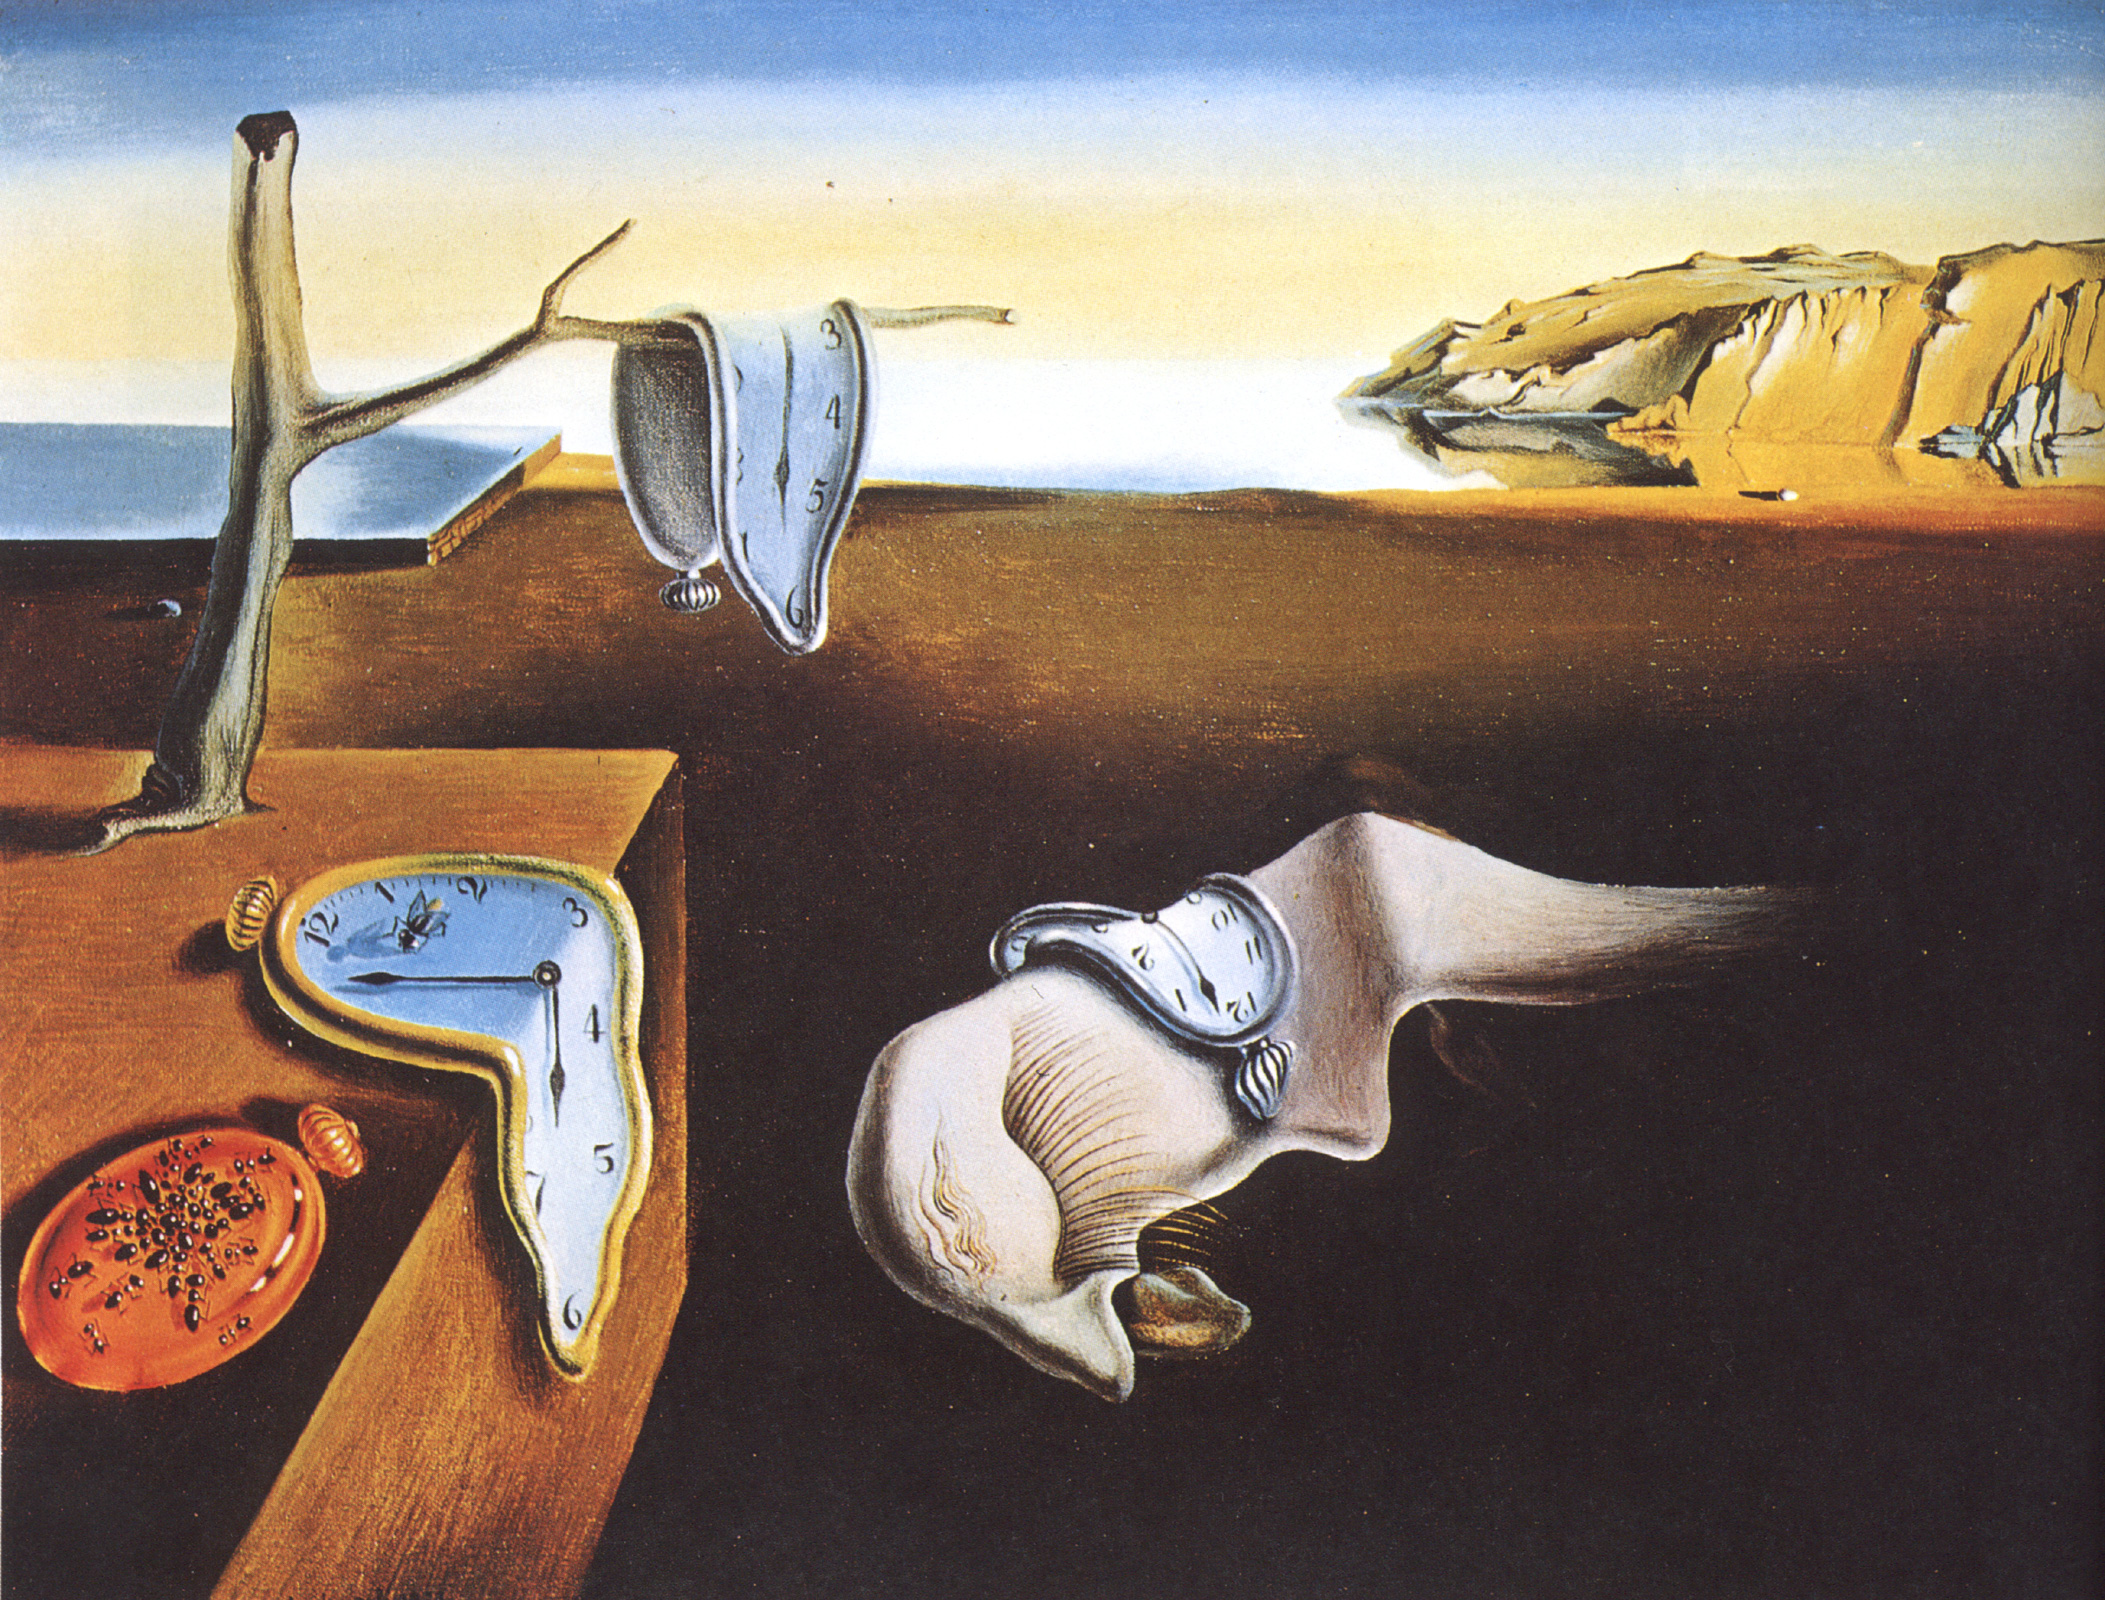
\includegraphics[scale=4.2]{frontpage}}} % Image background

\begin{tikzpicture}[remember picture, overlay]
\node[fill=white, fill opacity=0.6, anchor=north,minimum height=6cm, minimum width=\paperwidth] (names) at ([yshift=19cm]current page.south){};
\node[font=\normalfont\fontsize{35}{35}\sffamily\selectfont] at ([yshift=17cm]current page.south) {GridCal};
\node[font=\normalfont\fontsize{35}{35}\sffamily\selectfont \Huge] at ([yshift=15cm]current page.south) {Santiago Peñate Vera};
\end{tikzpicture}



%\centering
%%\vspace{5cm}
%\par\normalfont\fontsize{35}{35}\sffamily\selectfont
%\textbf{GridCal Manual }\\
%{\LARGE }\par % Book title
%\vspace*{1cm}
%{\Huge Santiago Peñate Vera}\par % Author name
%\endgroup

%----------------------------------------------------------------------------------------
%	COPYRIGHT PAGE
%----------------------------------------------------------------------------------------

\newpage
~\vfill
\thispagestyle{empty}

%\noindent Copyright \copyright\ 2014 Andrea Hidalgo\\ % Copyright notice

\noindent \textsc{GridCal}\\

\noindent Research oriented power systems software.\\ % License information

\noindent \textit{Started writing this document in Madrid the 9th of October of 2016} % Printing/edition date

%----------------------------------------------------------------------------------------
%	TABLE OF CONTENTS
%----------------------------------------------------------------------------------------

\chapterimage{chapterhdr1.jpg} % heading image

\pagestyle{empty} % No headers

\renewcommand\contentsname{Table of content}
%\renewcommand{\bibname}{Bibliography}
\tableofcontents% Print the table of contents itself

%\cleardoublepage % Forces the first chapter to start on an odd page so it's on the right

\pagestyle{fancy} % Print headers again

%----------------------------------------------------------------------------------------
%	CHAPTER 1
%----------------------------------------------------------------------------------------

\chapterimage{chapterhdr1.jpg} % Chapter heading image

\chapter{Introduction}

GridCal is a research oriented power systems software.  \newline

Research oriented? How? Well, it is a fruit of research. It is designed to be modular. As a researcher I found that the available software (not even talking about commercial options) are hard to expand or adapt to achieve complex simulations. GridCal is designed to allow you to build and reuse modules, which eventually will boost your productivity and the possibilities that are at hand. \newline

I have made other projects (even another open source one: fPotencia in C++). I believe that this project encapsulates my half life of programming experience and the curiosity I have developed for power systems. \newline

So, I do really hope you enjoy it, and if you have comments, suggestions or just want to collaborate, do not hesitate to contact.\newline

\begin{flushright}
	Cheers, 

Santiago
\end{flushright}


%----------------------------------------------------------------------------------------
%	CHAPTER 2
%----------------------------------------------------------------------------------------

\chapterimage{chapterhdr1.jpg} % Chapter heading image
\chapter{Structure}

GridCal uses an object oriented approach for all the data and simulation management. However the object orientation is very inefficient when used in numerical computation, that is why there are \verb|compile()| functions that extract the information out of the objects and turn this information into vectors, matrices and DataFrames in order to have efficient numerical computations. I have found this approach to be the best compromise between efficientcy and code escalability and maintainability after having been involved in quite some number-crunching software developments.

The whole idea can be summarized as:

\begin{verbatim}
Object oriented structures -> intermediate objects holding arrays -> Numerical modules
\end{verbatim}




\section{Circuit and MultiCircuit}

The concept of circuit should be easy enough to understand. It represents a set of nodes (buses) and branches (lines, transformers or other impedances)


The \verb|MultiCircuit| class is the main object in GridCal. It represents a circuit that may contain islands. It is important to understand that a circuit split in two or more islands cannot be simulated as is, because the admittance matrix would be singular. The solution to this is to split the circuit in island-circuits. Therefore \verb|MultiCircuit| identifies the islands and creates individual \verb|Circuit| objects for each of them.

As I said before GridCal uses an object oriented approach for the data management. This allows to group the data in a smart way. In GridCal I have decided to have only two types of object directly declared in a \verb|Circuit| or \verb|MultiCircuit| object. These are the \verb|Bus| and the \verb|Branch|. The branches connect the buses and the buses contain all the other possible devices like loads, generators, batteries, etc. This simplifies enormously the management of element when adding, associating and deleting.

\section{The Bus object}

The Bus object is the container of all the possible devices that can be attached to a bus bar or substation. Such objects can be loads, voltage controlled generators, static generators, batteries, shunt elements, etc.

\section{The branch object}


\section{Class diagram}

Here the API class diagram is sketched. All the classes are included but only the most fundamental properties and functions od each class are included to keep the diagram simple.

\begin{figure}[h]
	\centering
	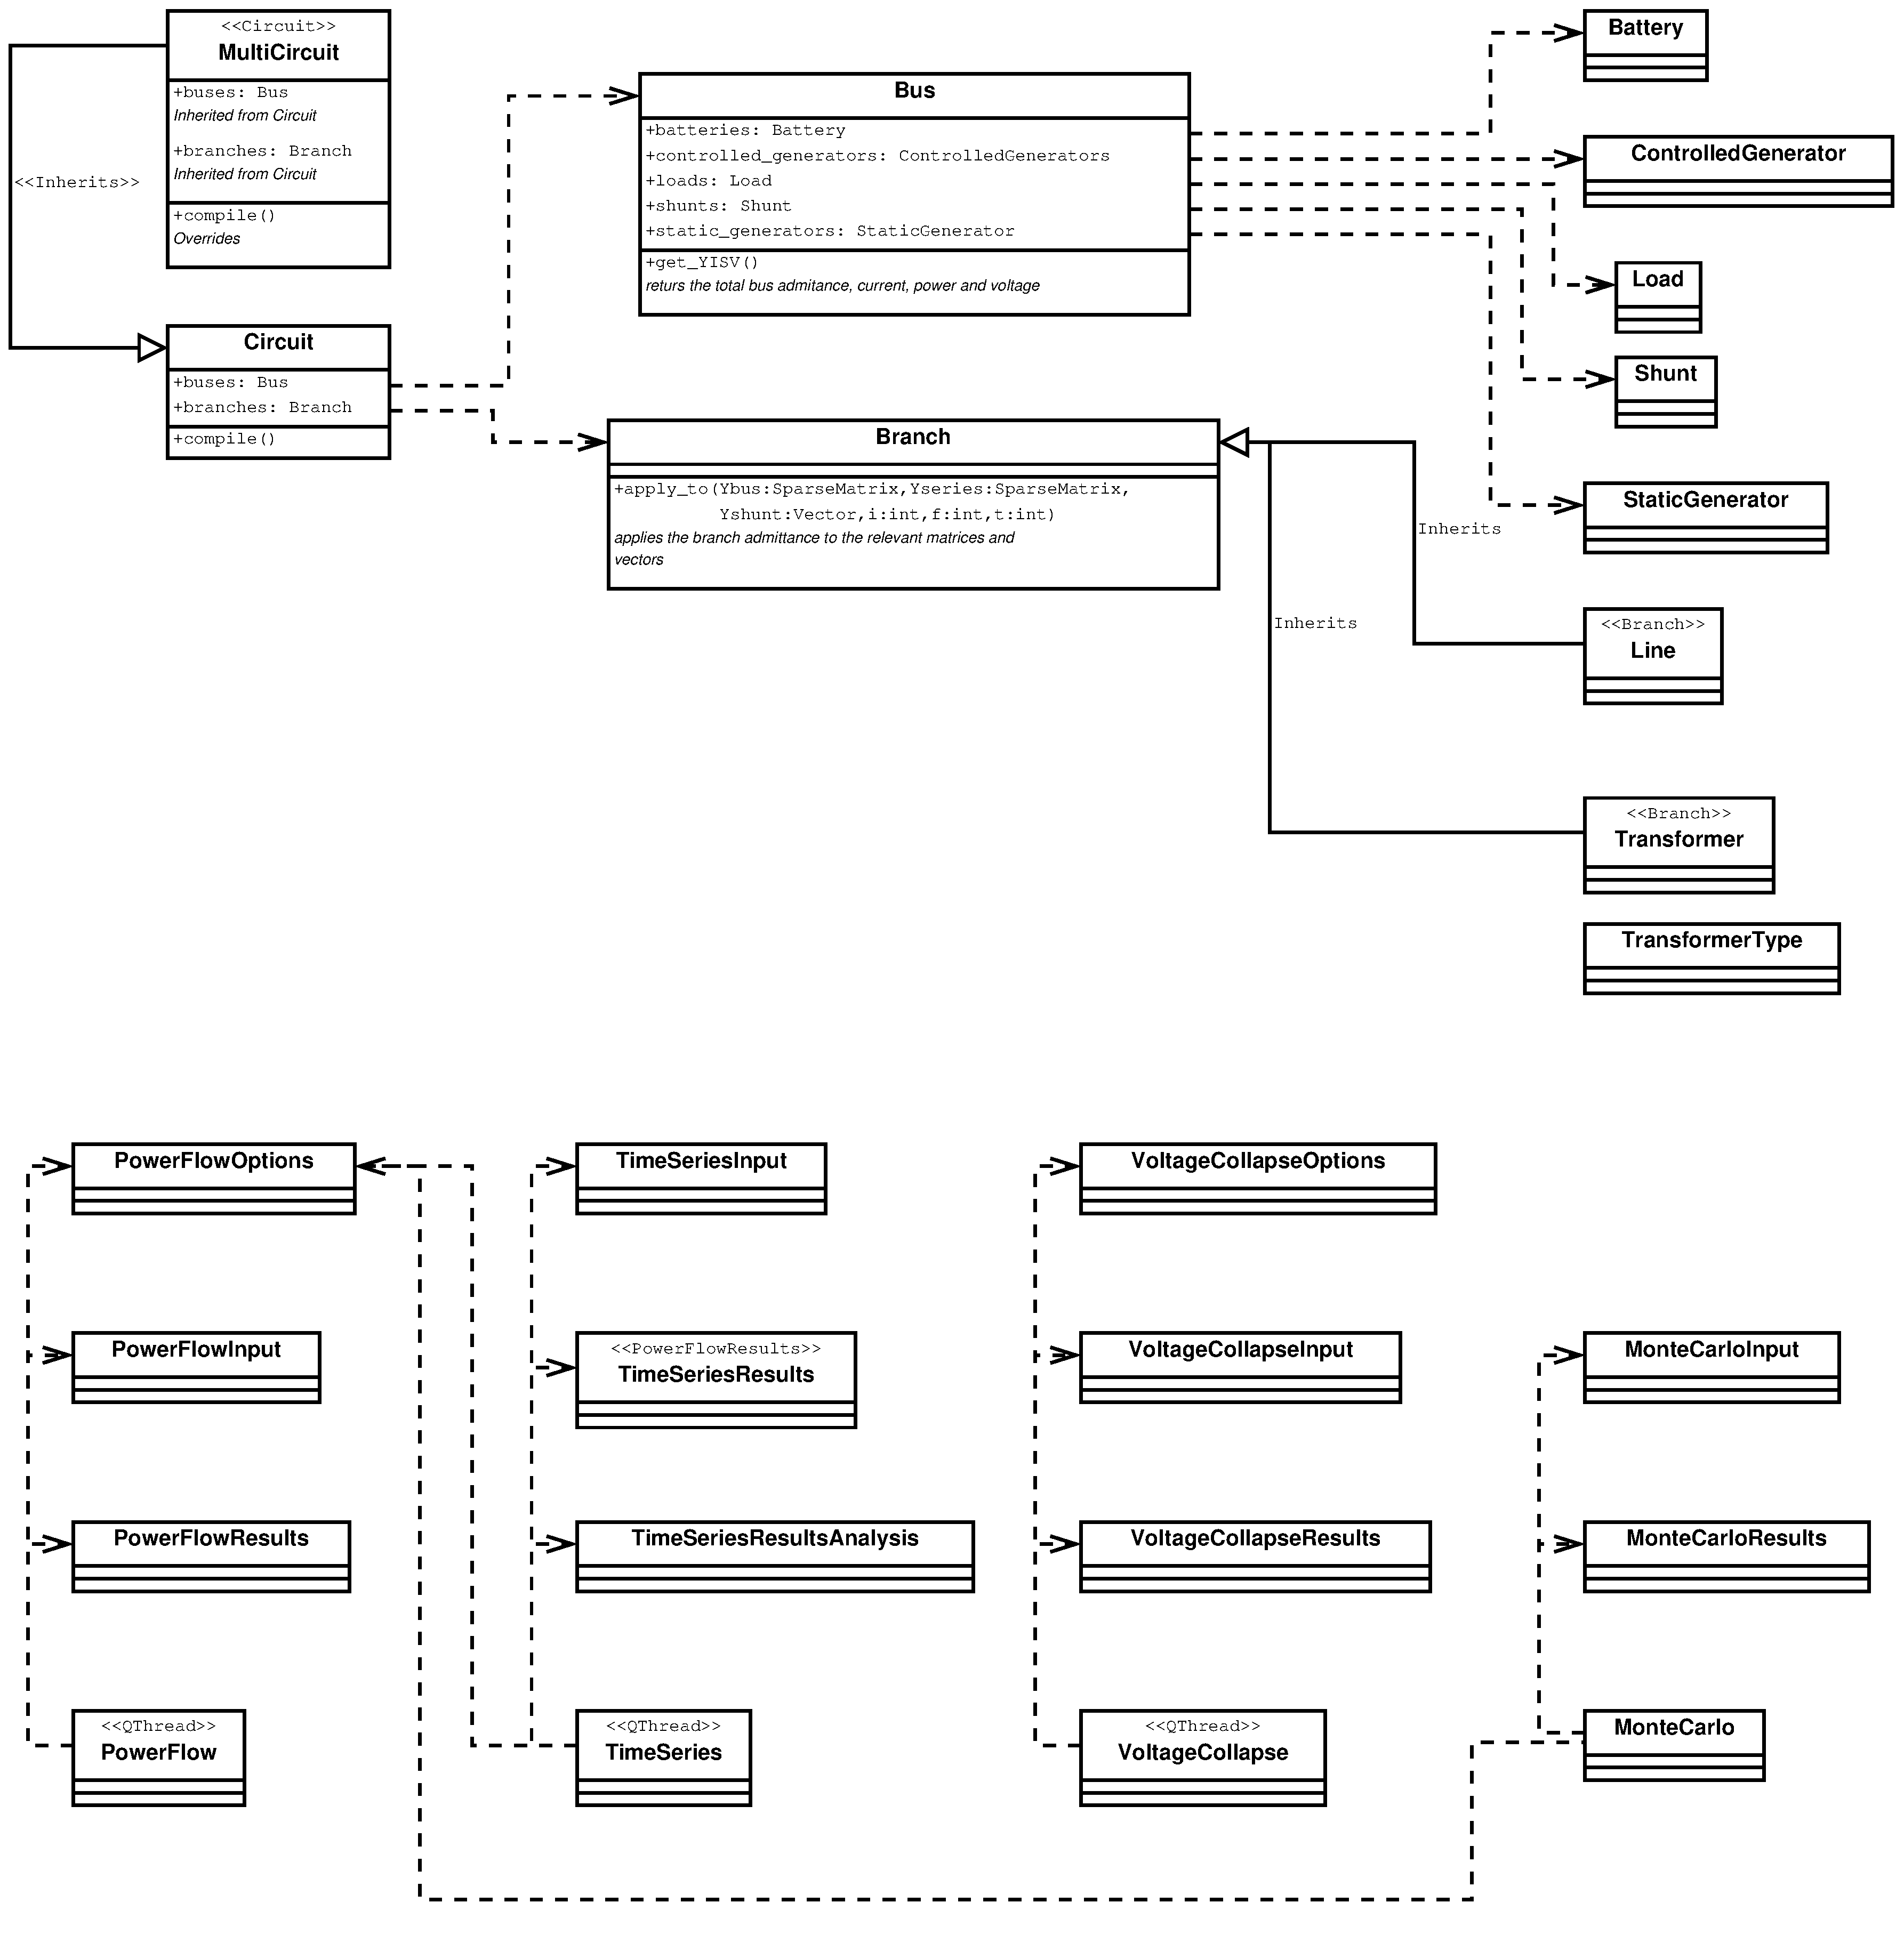
\includegraphics[width=1.0\linewidth]{ClassDiagram.eps}
	\caption{Simplified class diagram of GridCal's API}
	\label{fig:ClassDiagram}
\end{figure}

%----------------------------------------------------------------------------------------
%	CHAPTER 3
%----------------------------------------------------------------------------------------

\chapterimage{chapterhdr1.jpg} % Chapter heading image
\chapter{Models}



\section{Building the admittance matrices}

This operation occurs in the \verb|Compile()| function of the \verb|Circuit| object. This function compiles many other magnitudes and among them \verb|Ybus|, \verb|Yseries| and \verb|Yshunt|.

\begin{itemize}
	\item \verb|Ybus|: Complete admittance matrix.
	
	It is a sparse matrix of size $n \times n$
	
	\item \verb|Yseries|: Admittance matrix of the series elements. It contains no value comming from shunt elements or the shunt parts of the branch model.
	
	It is a sparse matrix of size $n \times n$
	
	\item \verb|Yshunt|: Admittance vector of the shunt elements and the shunt parts of the branch model. 
	
	It is a vector of size $n$
	
	\item \verb|Yf|: Admittance matrix of the banches with their \textit{from} bus.
	
	It is a sparse matrix of size $m \times n$
	 
	\item \verb|Yt|: Admittance matrix of the banches with their \textit{to} bus.
	
	It is a sparse matrix of size $m \times n$\newline
\end{itemize}

Where $n$ is the number of buses and $m$ is the number of branches.

The relation between the admittance matrix and the series and shunt admittance matrices is the following:
\begin{equation}
Y_{bus} = Y_{series} + Y_{shunt}
\end{equation}

The algorithmic logic to build the matrices in pseudo code is the following:

\begin{verbatim}
n = number of buses in the circuit
m = number of branches in the circuit
For i=0 to n:
   bus_shunt_admittance, bus_current, bus_power, bus_voltage = buses[i].get_YISV()
   
   Yshunt[i] = bus_shunt_admittance
end

For i=0 to m:
   f = get_bus_inde(branches[i].bus_from)
   t = get_bus_inde(branches[i].bus_to)
   
   // the matrices are modified by the branch object itself
   branches[i].apply_to(Ybus,Yseries,Yshunt,Yf,Yt,i,f,t)
end
	
\end{verbatim}

\section{The universal branch model}

The following describes the model that is applied to each type of admittance matrix in the \verb|apply_to()| function inside the \verb|Branch| object seen before.

The model implemented to describe the behavior of the transformers and lines is the $\pi$ (pi) model.
\begin{figure}[h]
	\centering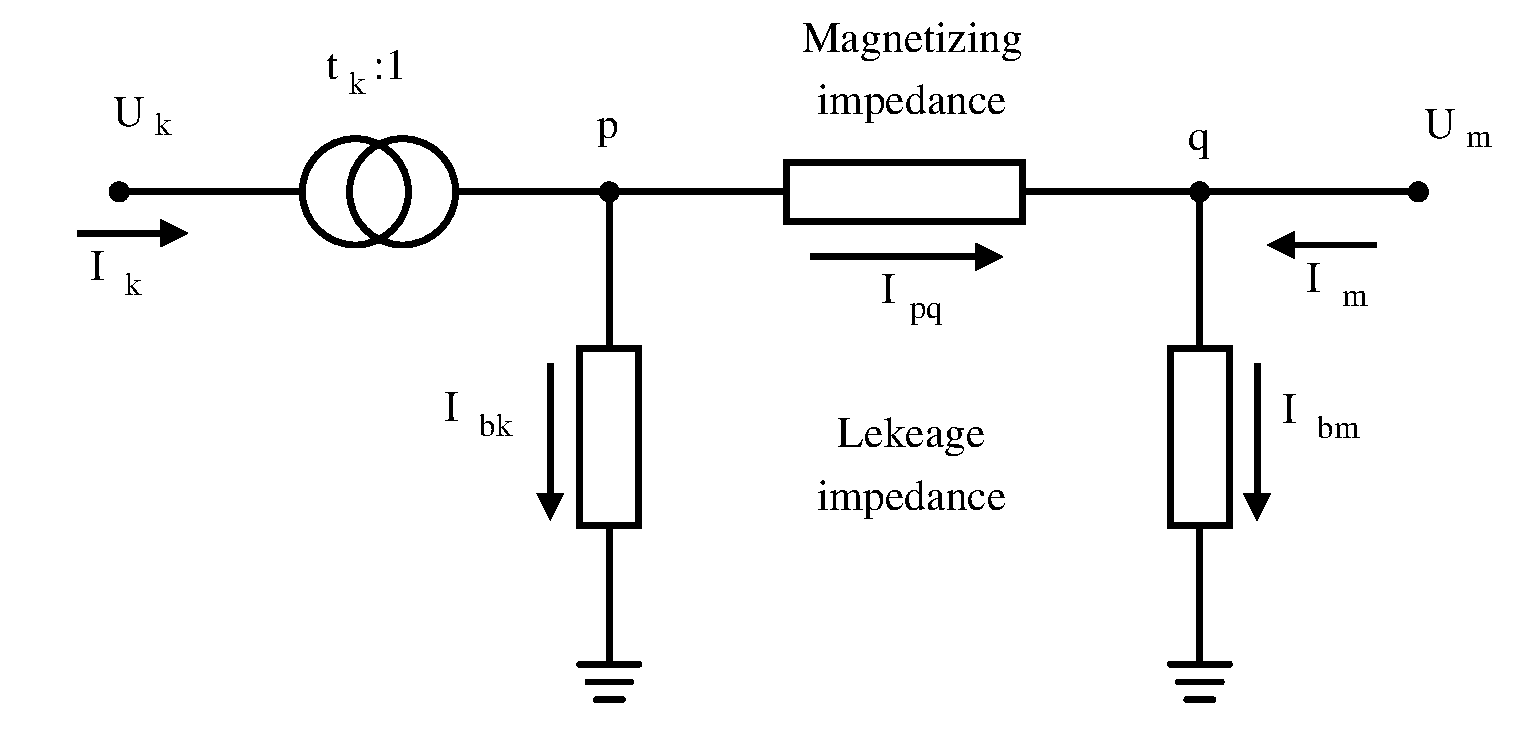
\includegraphics[width=0.8\linewidth]{pi-trafo.eps}
	\caption{$\pi$ model of a branch}
	\label{trafo pi model}
\end{figure}

To define the $\pi$ branch model we need to specify the following magnitudes:

\begin{itemize}
	\item $z_{series}$: Magnetizing impedance or simply series impedance. It is given in p.u.
	\item $y_{shunt}$: Leakage impedance or simply shunt impedance. It is given in p.u.
	\item $tap\_module$: Module of the tap changer. It is a magnitude around 1.
	\item $tap\_angle$: Angle of the tap changer. Angle in radians.\newline
\end{itemize}


%tap = self.tap_module * exp(-1j * self.angle)

In order to apply the effect of a branch to the admittance matrices, first we compute the complex tap value.
$$tap = tap\_module \cdot e^{-j \cdot tap\_angle}$$  

Then we compose the equivalent series and shunt admittance values of the branch. Both values are complex.
%Ys = 1 / self.z_series
$$Y_s = \frac{1}{z_{series}}$$
%Ysh = self.y_shunt / 2
$$Y_{sh} = \frac{y_{shunt}}{2}$$

\begin{itemize}
	\item $z_{series}$: Series impedance of the branch composed by the line resistance and its inductance. $z_{series}=r + jl$
	
	\item $y_{shunt}$: Shunt admittance of the line composed by the conductance and the susceptance. $y_{shunt}=c+jb$\newline
\end{itemize}



The general branch model is represented by a $2 \times 2$ matrix.
$
Y_{branch}=\left( \begin{array}{ccc}
Y_{ff} & Y_{ft} \\
Y_{tf} & Y_{tt} \end{array} \right)
$

In this matrix, the elements are the following:

%Yff = Ytt / (tap * conj(tap))
%Yft = - Ys / conj(tap)
%Ytf = - Ys / tap
%Ytt = Ys + Ysh

$$Y_{ff} = \frac{Y_s + Y_{sh}}{tap \cdot conj(tap)}  $$
$$Y_{ft} = - Y_s / conj(tap)$$
$$Y_{tf} = - Y_s / tap$$
$$Y_{tt} = Y_s + Y_{sh}$$

\subsubsection{Ybus}

The branch admittance values are applied to the complete admittance matrix as follows:

%Ybus[f, f] += Yff
%Ybus[f, t] += Yft
%Ybus[t, f] += Ytf
%Ybus[t, t] += Ytt
$${Y_{bus}}_{f, f} = {Y_{bus}}_{f, f}  + Y_{ff}$$
$${Y_{bus}}_{f, t} = {Y_{bus}}_{f, t} + Y_{ft}$$
$${Y_{bus}}_{t, f} = {Y_{bus}}_{t, f} + Y_{tf}$$
$${Y_{bus}}_{t, t} = {Y_{bus}}_{t, t} + Y_{tt}$$


These formulas assume that there might be something already in $Y_{bus}$, therefore the right way to modify these values is to add the own branch values.


\subsection{Yshunt}
%Yff_sh = Ysh
%Ytt_sh = Yff_sh / (tap * conj(tap))
%Yshunt[f] += Yff_sh
%Yshunt[t] += Ytt_sh
$${Y_{shunt}}_f = {Y_{shunt}}_f  + Y_{sh}$$
$${Y_{shunt}}_t = {Y_{shunt}}_t  + \frac{Y_{sh}}{tap \cdot conj(tap)}$$

\subsection{Yseries}
%Yseries[f, f] += Ys / (tap * conj(tap))
%Yseries[f, t] += Yft
%Yseries[t, f] += Ytf
%Yseries[t, t] += Ys

$${Y_{series}}_{f, f} = {Y_{series}}_{f, f}  + \frac{Y_{s}}{tap \cdot conj(tap)}$$
$${Y_{series}}_{f, t} = {Y_{series}}_{f, t} + Y_{ft}$$
$${Y_{series}}_{t, f} = {Y_{series}}_{t, f} + Y_{tf}$$
$${Y_{series}}_{t, t} = {Y_{series}}_{t, t} + Y_{s}$$

\subsection{Yf and Yt}
%# Yf = csr_matrix((r_[Yff, Yft], (i, r_[f, t])), (nl, nb))
%# Yt = csr_matrix((r_[Ytf, Ytt], (i, r_[f, t])), (nl, nb))

%Yf[i, f] += Yff  # Ybus[f, f]
%Yf[i, t] += Yft  # Ybus[f, t]
$${Y_f}_{i, f} = {Y_f}_{i, f} + Y_{ff}$$
$${Y_f}_{i, t} = {Y_f}_{i, t} + Y_{ft}$$

%Yt[i, f] += Ytf  # Ybus[t, f]
%Yt[i, t] += Ytt  # Ybus[t, t]
$${Y_t}_{i, f} = {Y_t}_{i, f} + Y_{tf}$$
$${Y_t}_{i, t} = {Y_t}_{i, t} + Y_{tt}$$


\section{The transformer definition from the short circuit test values}

The transformers are modeled as $\pi$ branches too. In order to get the series impedance and shunt admittance of the transformer to match the branch model, it is advised to transform the specification sheet values of the device into the desired values. The values to take from the specs sheet are:
\begin{itemize}
	\item $S_n$: Nominal power in MVA.
	\item $U_{hv}$: Voltage at the high-voltage side in kV.
	\item $U_{lv}$: Voltage at the low-voltage side in kV.
	\item $U_{sc}$: Short circuit voltage in \%.
	\item $P_{cu}$: Copper losses in kW.
	\item $I_0$: No load current in \%.
	\item $GX_{hv1}$: Reactance contribution to the HV side. Value from 0 to 1.
	\item $GR_{hv1}$: Resistance contribution to the HV side Value from 0 to 1.\newline
\end{itemize}

Then, the series and shunt impedances are computed as follows:

Nominal impedance HV (Ohm): $Zn_{hv} = U_{hv}^2 / S_n$ \newline


Nominal impedance LV (Ohm): $Zn_{lv} = U_{lv}^2 / S_n$ \newline


Short circuit impedance (p.u.): $z_{sc} = U_{sc} / 100$\newline

Short circuit resistance (p.u.): $r_{sc} = \frac{P_{cu} / 1000}{S_n}$\newline

Short circuit reactance (p.u.): $x_{sc} = \sqrt{z_{sc}^2 - r_{sc} ^2}$\newline


HV resistance (p.u.): $r_{cu,hv} = r_{sc} \cdot GR_{hv1}$\newline


LV resistance (p.u.): $r_{cu,lv} = r_{sc} \cdot (1 - GR_{hv1})$\newline


HV shunt reactance (p.u.): $xs_{hv} = x_{sc} \cdot GX_{hv1}$\newline


LV shunt reactance (p.u.): $xs_{lv} = x_{sc} \cdot (1 - GX_{hv1})$\newline

Shunt resistance (p.u.): $r_{fe} = \frac{Sn}{P_{fe} / 1000}$\newline


Magnetization impedance (p.u.): $z_m = \frac{1}{I_0 / 100}$\newline

Magnetization reactance (p.u.): $x_m = \frac{1}{\sqrt{\frac{1}{z_m^2} - \frac{1}{r_{fe}^2}}}$ \newline

If the content of the square root is negative, set the magnetization impedance to zero.\\


The final complex calculated parameters in per unit are:

Magnetizing impedance (or series impedance): $z_{series} = Z_m = r_{fe} +j \cdot x_m$

Leakage impedance (or shunt impedance): $Z_l = r_{sc} + j \cdot x_{sc}$

Shunt admittance: $y_{shunt} = 1 / Z_l$

%----------------------------------------------------------------------------------------
%	CHAPTER 4
%----------------------------------------------------------------------------------------

\chapterimage{chapterhdr1.jpg} % Chapter heading image
\chapter{Power flow methods}

\section{Newton-Raphson-Iwamoto}


\newpage
\section{Holomorphic Embedding (ASU)}

First introduced by Antonio Trias in 2012 \cite{TriasHELM}, promises to be a non-divergent power flow method. Trias originally developed a version with no voltage controlled nodes (PV), in which the convergence properties are excellent (With this software try to solve any grid without PV nodes to check this affirmation). 

The version programmed in the file \verb|HelmVect.py| has been adapted from the master thesis of Muthu Kumar Subramanian at the Arizona State University \cite{subramanian2014application}. This version includes a formulation of the voltage controlled nodes. My experience indicates that the introduction of the PV control deteriorates the convergence properties of the holomorphic embedding method. However, in many cases, it is the best approximation to a solution. especially when Newton-Raphson does not provide one.

The \verb|HelmVect.py|  file contains a vectorized version of the algorithm. This means that the execution in python is much faster than a previous version that uses loops.

\subsection{Concepts}

All the power flow algorithms until the HELM method was introduced were iterative and recursive. The helm method is iterative but not recursive. A simple way to think of this is that traditional power flow methods are exploratory, while the HELM method is a planned journey. In theory the HELM method is superior, but in practice the numerical degeneration makes it less ideal.

The fundamental idea of the recursive algorithms is that given a voltage initial point (1 p.u. at every node, usually) the algorithm explores the surroundings of the initial point until a suitable voltage solution is reached or no solution at all is found because the initial point is supposed to be "far" from the solution.

On the HELM methods, we form a "curve" that departures from a known mathematically exact solution that is obtained from solving the grid with no power injections. This is possible because with no power injections, the grid equations become linear and straight forward to solve. The arriving point of the "curve" is the solution that we want to achieve. That "curve" is best approximated by a Padè approximation. To compute the Padè approximation we need to compute coefficient of the unknown variables, in our case the voltage (and possibly the reactive power).

The HELM formulation consists in the derivation of formulas that enable the calculation of the coefficients of the series that describes the "curve" from the mathematically know solution to the unknown solution. Once the coefficients are obtained, the Padè approximation computes the voltage solution at the "end of the curve", providing the desired voltage solution. The more coefficients we compute the more exact the solution is (this is true until the numerical precision limit is reached).\newline 


All this sounds very strange, but it works ;)\newline 


If you want to get familiar with this concept, you should read about the homotopy concept. In practice the continuation power flow does the same as the HELM algorithm, it takes a known solution and changes the loading factors until a solution for another state is reached.

\subsection{Fundamentals}

The fundamental equation that defines the power flow problem is:
\begin{equation}
S = V \times (Y \times V + I)^*
\end{equation}

Most usefully represented like this:


\begin{equation}
{\textbf{Y} \times \textbf{V}} = \left(\frac{\textbf{S}}{\textbf{V}}\right)^* 
\label{base_eq}
\end{equation}


The holomorphic embedding is to insert a "travelling" parameter $\alpha$, such that for $\alpha=0$ we have an mathematically exact solution of the problem (but not the solution we're looking for...), and for $\alpha=1$ we have the solution we're looking for. The other thing to do is to represent the variables to be computes as McLaurin series. We'll go step by step.\newline

For $\alpha=0$ we say that $S=0$, in this way the equation \ref{base_eq} becomes linear, and its solution is mathematically exact. But for that to be useful in our case we need to split the admittance matrix $Y$ into $Y_{series}$ and $Y_{shunt}$

\begin{equation}
\textbf{Y}_{series} \times \textbf{V} = \left(\frac{\textbf{S}}{\textbf{V}}\right)^* - \textbf{Y}_{shunt} \times \textbf{V}
\label{base_eq_alpha_0}
\end{equation}

This is what will allow us to find the zero "state" in the holomorphic series calculation. For $\alpha=1$ we say that $S=S$, so we don't know the voltage solution, however we can determine a path to get there:

\begin{equation}
{\textbf{Y }\times \textbf{V}( \alpha )} = \left(\frac{ \alpha\textbf{S}}{\textbf{V}( \alpha )}\right)^* - \alpha \textbf{Y}_{shunt} \times \textbf{V}( \alpha ) = \frac{ \alpha\textbf{S}^*}{\textbf{V}( \alpha )^*} - \alpha \textbf{Y}_{shunt} \times \textbf{V}( \alpha )
\label{base_eq_embedded}
\end{equation}

Wait, what?? did you just made this stuff up??, well so far my reasoning is:
\begin{itemize}
	\item The voltage ($V$) is what I have to convert into a series, and the series depend of $\alpha$, so it makes sense to say that $V$ is now $V(\alpha)$.
	
	\item Regarding the $\alpha$ that multiplies the $S$, the power ($S$) is what I vary during the \textit{travel} from $\alpha=0$ to $\alpha=1$, so that is why it has to be accompanied by the \textit{traveling} parameter $\alpha.$
	
	\item In my opinion the $\alpha$ $\textbf{Y}_{shunt}$ is to provoke the first voltage coefficients to be one.  $\textbf{Y}_{series} \times \textbf{V}[0] = 0$, makes $V[0]=1$, and this is essential for later steps (to be able to use Padè). \newline
\end{itemize}

The series are expressed as McLaurin equations::

\begin{equation}
V(\alpha) = \sum_{n}^{\infty} V_n \alpha ^n
\end{equation}

There's still something to do. The magnitude $\left(\textbf{V}( \alpha )\right)^*$ has to be converted into $\left(\textbf{V}( \alpha^* )\right)^*$. This is done in order to make the function be actually holomorphic. The holomorphicity condition is tested by the Cauchy-Riemann condition, this is $\partial V / \partial \alpha^* = 0$, let's check that:



\begin{equation}
\partial \left(\textbf{V}( \alpha )^*\right) / \partial \alpha^*  = \partial \left(\sum_{n}^{\infty} V_n^* (\alpha ^n)^*\right) / \partial \alpha^*  = \sum_{n}^{\infty} \alpha ^n V_n^* (\alpha ^{n-1})^*
\end{equation} 
Which is not zero, obviously. Now with the proposed change:

\begin{equation}
\partial \left( \textbf{V}( \alpha^* )\right)^* / \partial \alpha^*  = \partial \left(\sum_{n}^{\infty} V_n^* (\alpha ^n)\right) / \partial \alpha^*  = 0
\end{equation} 

Yay!, now we're mathematically happy, since this stuff has no effect in practice because our $\alpha$ is not going to be a complex parameter, but for sake of being correct the equation is now:

\begin{equation}
{\textbf{Y}_{series}\times \textbf{V}( \alpha )} = \frac{ \alpha\textbf{S}^*}{\textbf{V}^*( \alpha^* )} - \alpha \textbf{Y}_{shunt} \times \textbf{V}( \alpha )
\label{base_eq_embedded2}
\end{equation}



%----------------------------------------------------------------------------------------
%	CHAPTER 4
%----------------------------------------------------------------------------------------

\chapterimage{chapterhdr1.jpg} % Chapter heading image
\chapter{Graphical User Interface}

% ----------------------------------------------------------------------------------------
% 	BIBLIOGRAPHY
% ----------------------------------------------------------------------------------------
%\chapter*{Bibliography}
\bibliographystyle{abbrv}
\bibliography{bibliography}

\end{document}